\chapter{Testing}
\section{Test Procedure}
\subsection{Overall System}
\label{sec:overallSystemTesting}

Three different tests will be done to test the overall system. To run these
tests a square wave and a sinusoid wave will be produced using a signal
generator at \SI{100}{\Hz}, \SI{1}{\kHz}, \SI{2}{\kHz}, \SI{5}{\kHz} and
\SI{10}{\kHz}. The signal generator has an accuracy of 2 decimal places, or
between \SI{1}{\Hz} and \SI{100}{\Hz} in this test. While the error is not
explicitly stated, the signal generator is a commercial product so the error
will be less than \SI{1}{\Hz} (the accuracy).

To reduce error, all measurements will be repeated 3 times and an average value
found and recorded. While the oscilloscope has a high enough impedance,
capacitance and inductance that they may have an effect on the test signal, the
signal generator will take this into account when calculating the signal
frequency.

The sinusoid wave will be fed into the oscilloscope at each different frequency,
and the time period and amplitude recorded from the waveform view. These will be
compared to the known values to compute an accuracy value for the oscilloscope.
Data will be recorded in~\cref{tab:analogueWaveData}.

\begin{table}
  \centering
  \begin{tabular}{SSSSSS}
    \toprule
      \multicolumn{3}{c}{Frequency (\si{\kHz})}&\multicolumn{3}{c}{Amplitude (\si{\V})}\\
      \cmidrule(lr){1-3} \cmidrule(lr){4-6}
      {Actual} & {Measured} & {\% error} & {Actual} & {Measured} & {\% error}\\
      \midrule

      0.101 & 0.0963 & 4.65\% & 4.9 & 4.8 & 2.04\% \\
      1.01 & 1.01 & 0.00\% & 4.9 & 4.8 & 2.04\% \\
      1.99 & 2.04 & 2.51\% & 4.9 & 4.7 & 4.08\% \\
      5.01 & 5.11 & 2.00\% & 4.9 & 4.8 & 2.04\% \\
      10.1 & 10.1 & 0.00\% & 4.9 & 4.8 & 2.04\% \\


      \bottomrule
  \end{tabular}
  \caption{Results from analogue wave testing}
  \label{tab:analogueWaveData}
\end{table}

Similarly, the square wave will be fed into the oscilloscope and the time period
recorded from the digital view. This will be compared to the known value to
compute an accuracy value, and data will be recorded
in~\cref{tab:digitalWaveData}.

\begin{table}
  \centering
  \begin{tabular}{SSS}
    \toprule

    \multicolumn{3}{c}{Frequency (\si{\kHz})}\\
    \cmidrule(lr){1-3}
    
    {Actual} & {Measured} & {\% error} \\

    \midrule

    0.100 & 0.110 & 10.0\% \\
    1.06 & 1.00 & 5.66\% \\
    2.00 & 2.02 & 1.00\% \\
    4.99 & 4.43 & 11.2\% \\
    10.0 & 8.40 & 16.0\%\\
    \bottomrule
  \end{tabular}
  \caption{Results from digital wave testing}
  \label{tab:digitalWaveData}
\end{table}

The square wave was also fed into the analogue input and the scope switched to
spectrum mode. As seen
in~\cref{fig:actualSquareSpectrum} the spectrum
looked exactly as one would expect for a square wave signal (based on the
prediction made from~\cref{sec:squareWaveFourierSeries}).

\begin{figure}[h]
  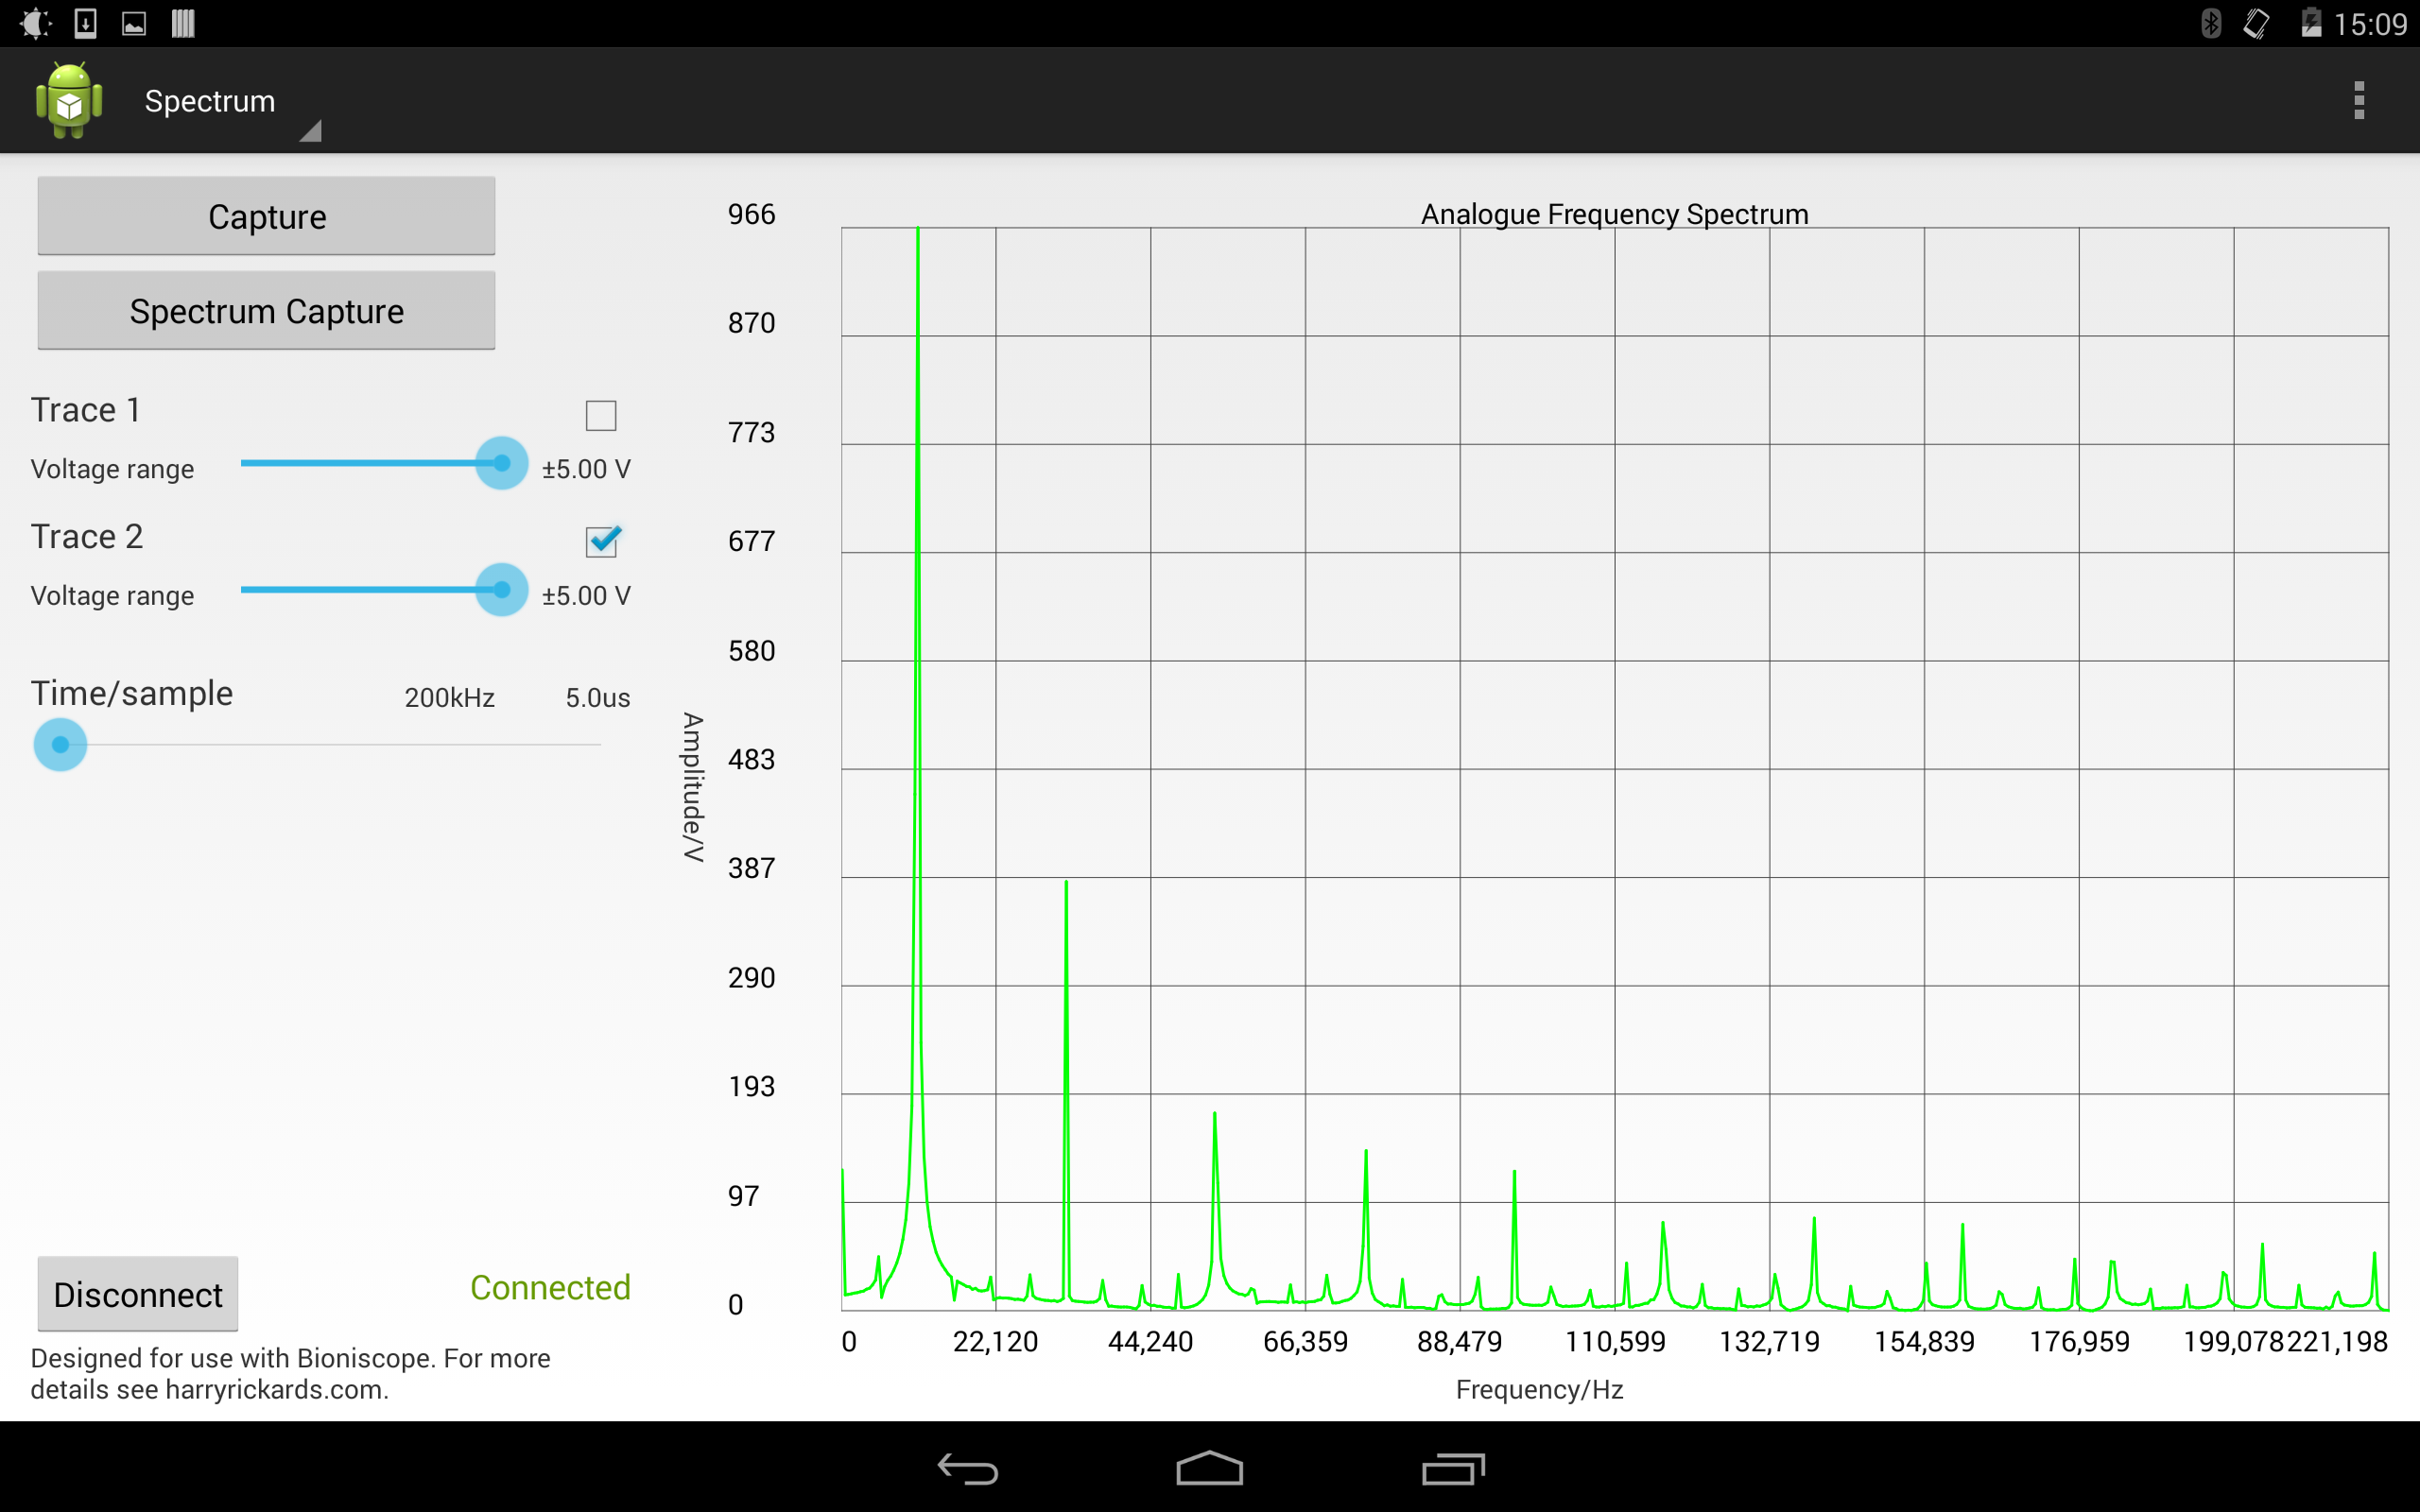
\includegraphics[width=\linewidth]{img/screenshots/spectrum.png}
  \caption{Frequency spectrum of square wave, as expected}
  \label{fig:actualSquareSpectrum}
\end{figure}

\subsubsection{Results}

Looking at the data above, error values are reasonably consistent so there are
no outliers that need to be taken care of.

Taking means, we find the average error to be 8.8\% for the digital wave and 1.8\%
for the analogue wave. While this would probably not be accurate enough for a
commercial product, it is certainly accurate enough for this project. Besides,
while some of the error undoubtedly comes from inaccuracies in the time delay
code (it has to delay to the nearest whole multiple of \SI{62.5}{\ns} as the
microcontroller uses a \SI{16}{\MHz} clock), the error could almost certainly be
significantly reduced by using compnents with stricter tolerance values (some
are 10\% at the moment).

\subsection{Initial Criteria}
\label{sec:initialCriteriaMet}

Next, the system needs to be checked to ensure it meets the numerical parameters
specified in~\cref{sec:numericalParameters}.

\subsubsection*{Frequency}
As seen above in~\cref{sec:overallSystemTesting}, the oscilloscope is accurate
and copes with a \SI{10}{\kHz} wave as required by the system.

\subsubsection*{Bandwidth}
To check the analogue bandwidth of the system, a \SI{1}{\MHz} square wave will be
produced using a signal generator. This will be input into the oscilloscope,
and a traditional CRO used to measure the output from the analogue circuitry.
Using the figures and working detailed in~\cref{sec:oscilloscopeSquare} we can
compare the visual output to calculate the total bandwidth of the system.

The bandwidth of the CRO is already known to be approximately \SI{20}{\MHz}
(from~\cref{sec:overallSystemTesting}) so provided the calculated bandwidth is
less than \SI{20}{\MHz} we know this is the analogue bandwidth of the
oscilloscope. If it's \SI{20}{\MHz} we know the analogue bandwidth is at least
\SI{20}{\MHz} and hence greater than our requirement of \SI{1}{\MHz}
(from~\cref{sec:numericalParameters}).

As we're counting discrete harmonics here, the frequency of the generated signal
simply needs to be at least 50\% accurate to ensure 100\% accuracy for the
number of harmonics. As a commercial signal generator will be used, it will
certainly reach this level of accuracy. The final answer for the bandwidth will
be accurate to within 1 harmonic of the fundamental frequency. While this is a
significant error, there's no way to reduce this error value without using
specialist equipment (i.e., a traditional RF spectrum analyser) or significantly
increasing the complexity of the test. As we only need to verify the bandwidth
is greater than \SI{1}{\MHz}, this is accurate enough for our purposes.

When the experiment was performed, the CRO showed the output seen in
\cref{fig:scopeBandwidthPhoto}. As
can be seen by comparing to~\cref{fig:squareWaveApproximations}, the square wave
is present to significantly more than the eleventh harmonic. So the bandwidth is
greater than \SI{11}{\MHz}, more than meeting the initial numerical parameters
(which specified \SI{1}{\MHz}).

\begin{figure}[h]
  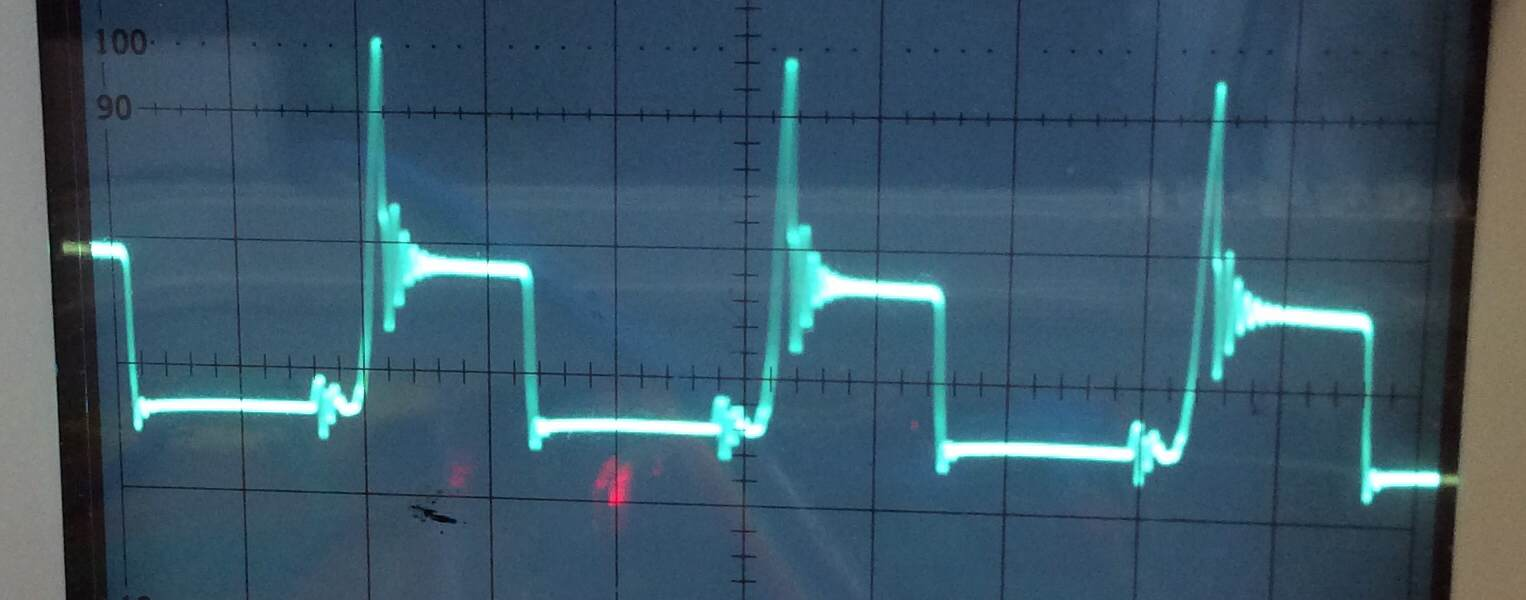
\includegraphics[width=\linewidth]{img/bw.jpg}
  \caption{The bandwidth-constrained square wave after passing through the analogue circuitry}
  \label{fig:scopeBandwidthPhoto}
\end{figure}

\section{Initial Assessment of System}

As discussed above, the system met all initial quantitative criteria. However,
while performing the above tests a critical issue was discovered.

Whenever the input signal fell below \SI{0}{\V}, the output from the analogue
circuitry was clipping.  Upon further investigation, it was discovered this was
because the digital potentiometer can only cope with voltages between \SI{0}{\V}
and $V_{SS}$ --- not those below \SI{0}{\V}.

Despite this, the oscilloscope still performed accurately and met the rest of
it's goals. While at this stage it did have limited usefuleness for analogue
signals (as a large number of analogue signals fall below \SI{0}{\V}), this did
not impede the digital performance of the oscilloscope.

To overcome this issue, an op amp circuit was set up to scale a signal by
$\frac{1}{2}$ and add on an offset of \SI{2.5}{\V}. This was implemented using a
standard noninverting summing amplifier, as shown
in~\cref{fig:introCircuitDiagram,fig:introCircuitPhoto}.

\begin{figure}[h]
  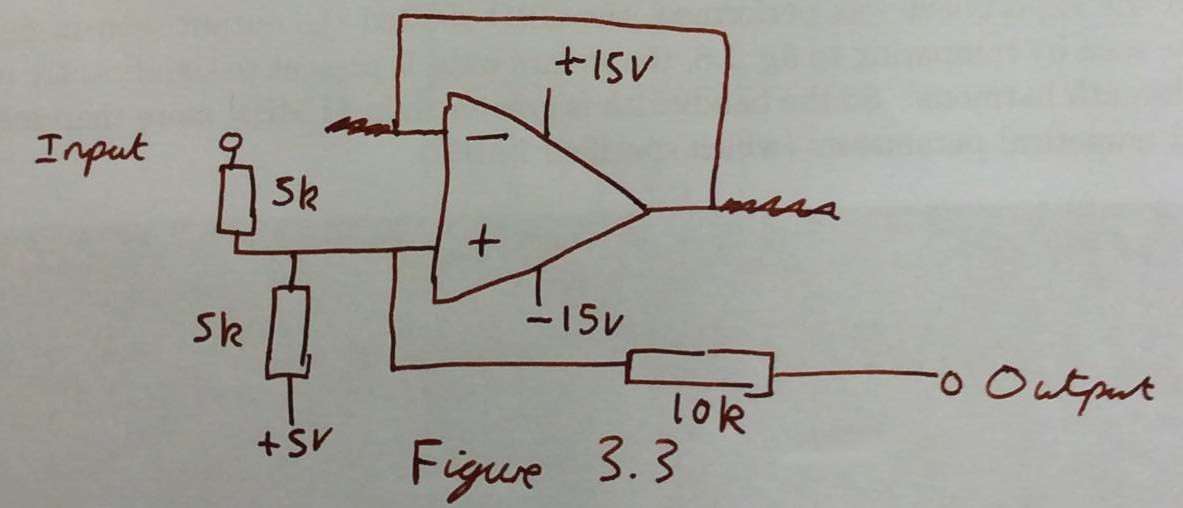
\includegraphics[width=\linewidth]{img/introCircuitDiagram.jpg}
  \caption{Circuit diagram for the op amp circuit added to fix the issue with negative signals}
  \label{fig:introCircuitDiagram}
\end{figure}

\begin{figure}[h]
  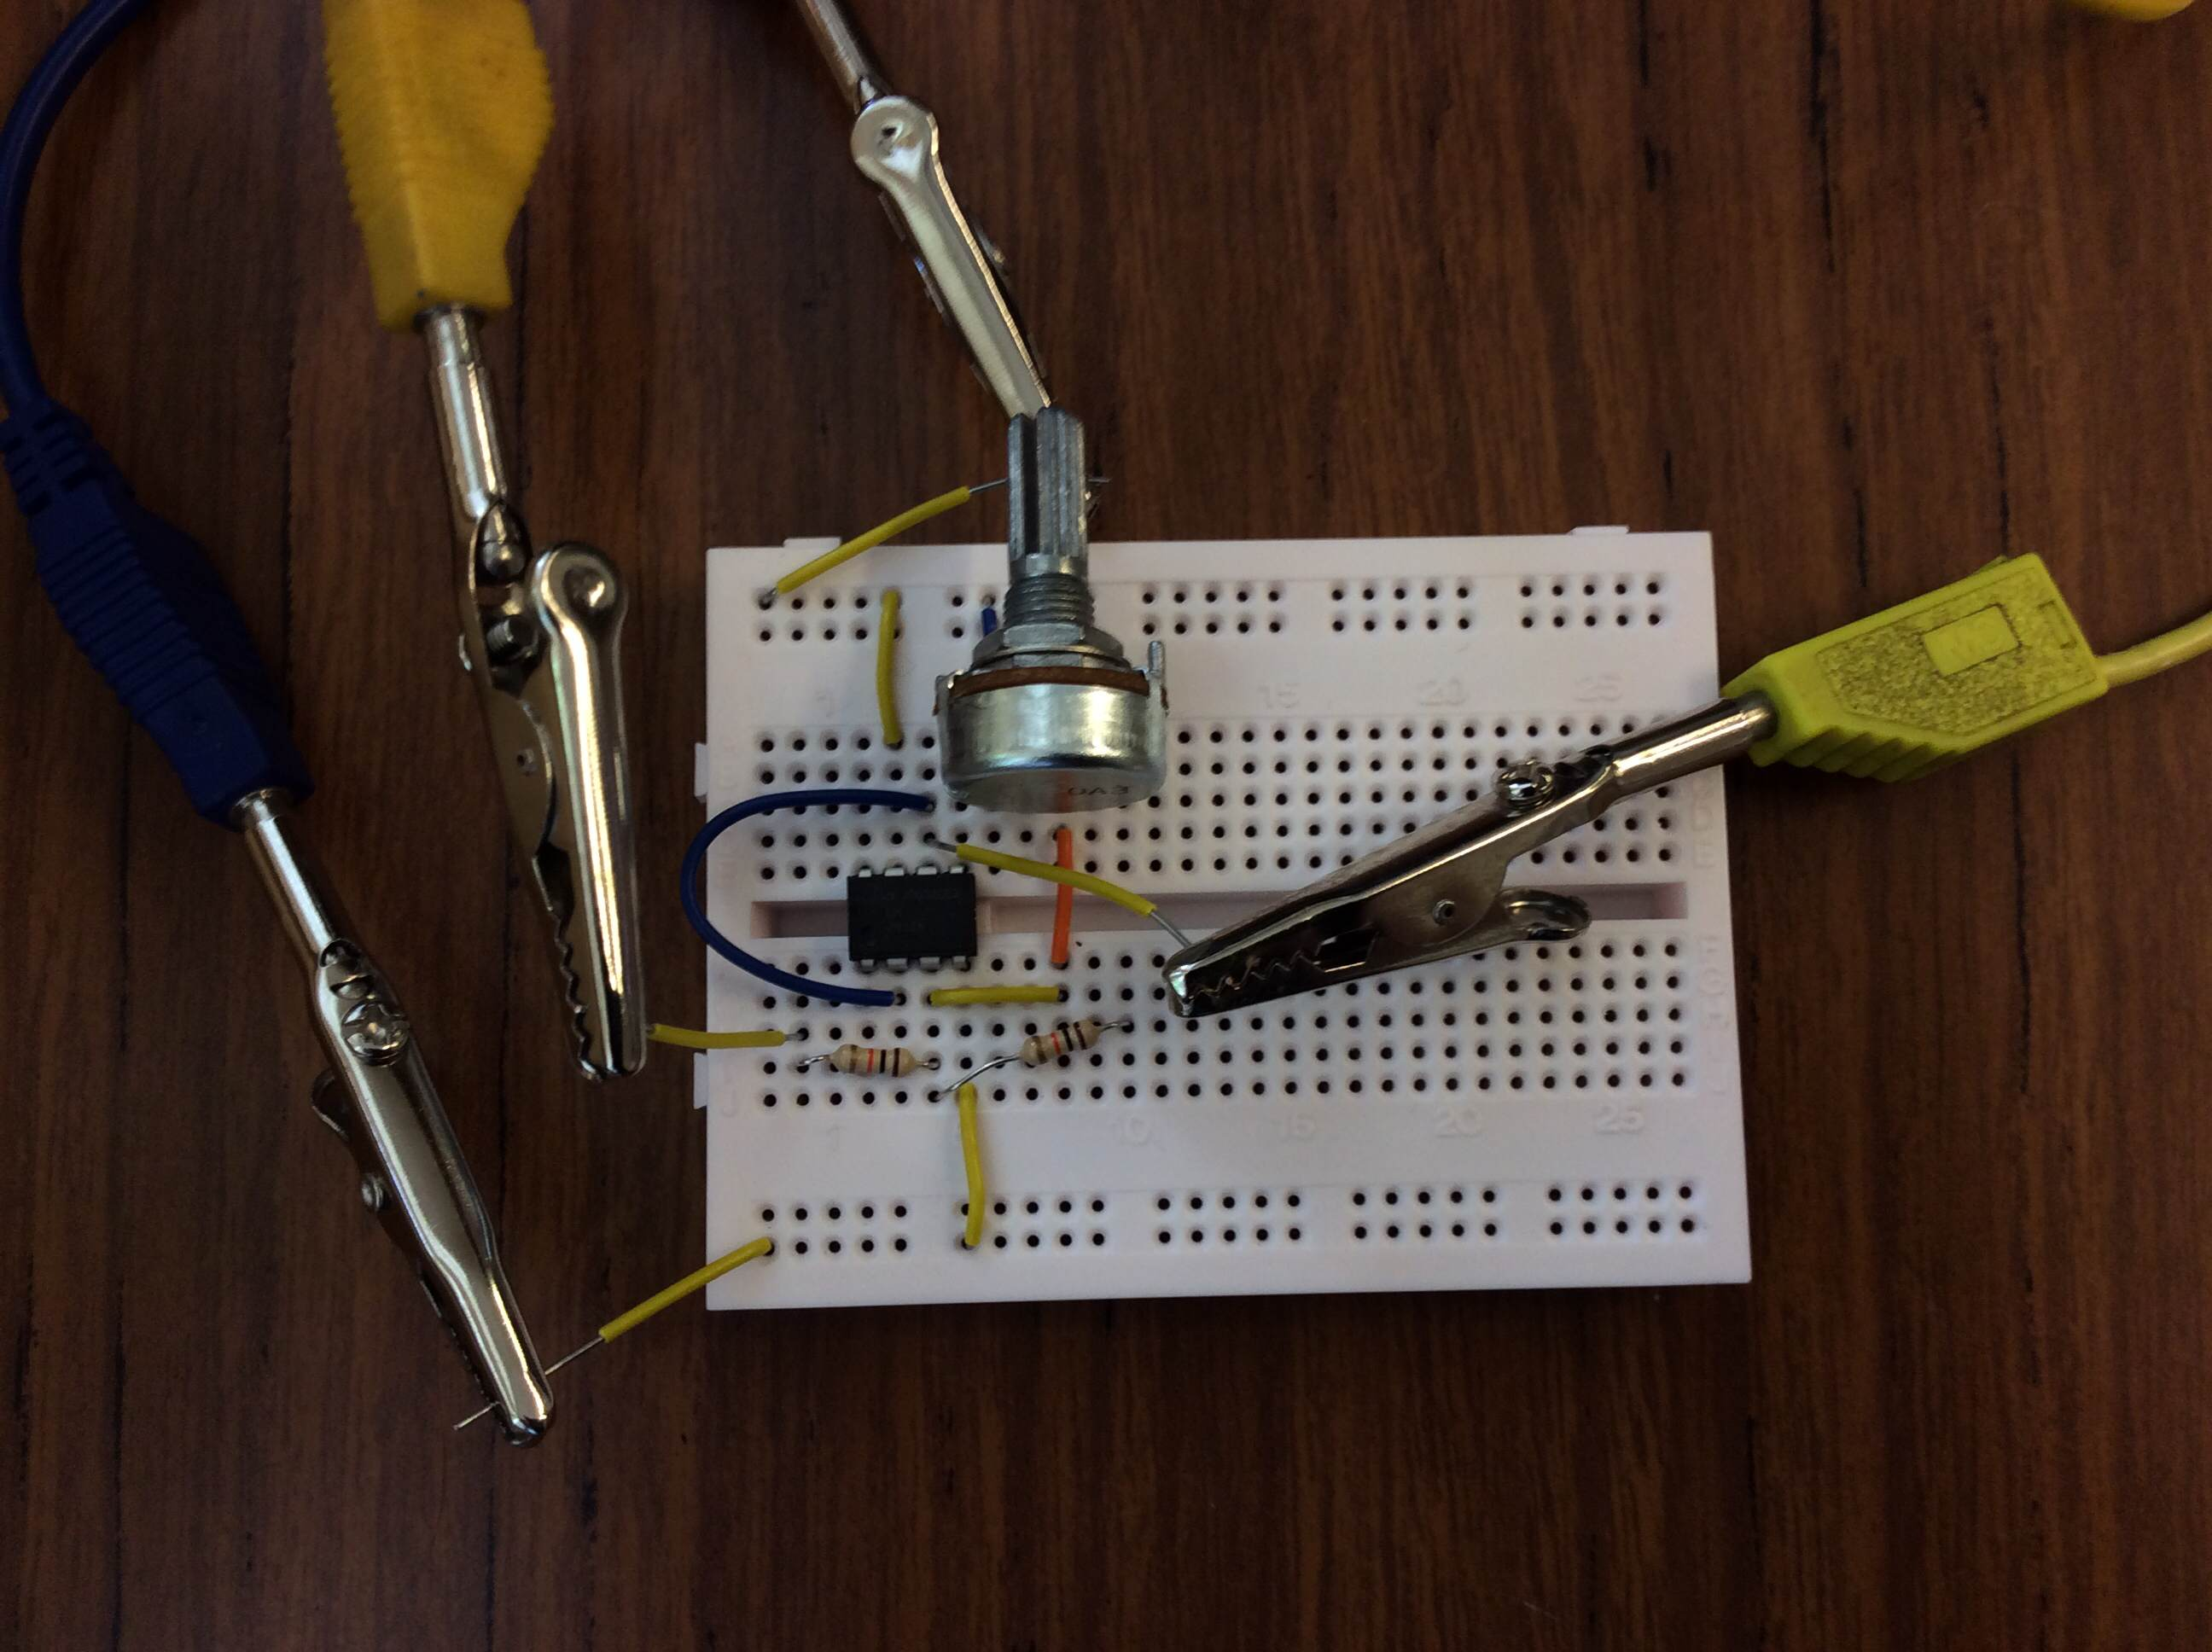
\includegraphics[width=\linewidth]{img/introCircuitPhoto.jpg}
  \caption{Breadboard photo of the op amp circuit added to fix the issue with negative signals}
  \label{fig:introCircuitPhoto}
\end{figure}

Now when testing the oscilloscope with signals that fell below \SI{0}{\V} it
worked fine. At this point, the system met all quantitative criteria and also
met the aim of the project: to produce a digital sampling oscilloscope that also
provided basic spectrum analysis and logic analyser functionality.
